\section{Evaluation Benchmarks and Model Synthesis}
\label{sec:benchmarks}

\begin{table*}[t]
\centering
\caption{Comprehensive Synthesis of Verified Scientific Multimodal Time Series Foundation Models and Reasoning Systems.}
\label{tab:foundation_models_summary}
\scriptsize
\resizebox{\textwidth}{!}{%
\begin{tabular}{@{}lp{2.0cm}p{3.0cm}p{3.4cm}cccp{3.0cm}@{}}
\toprule
\textbf{Model} & \textbf{Domain} & \textbf{Architectural Backbone} & \textbf{Pretraining Corpus \& Scale} & \textbf{Resolution} & \textbf{Physics Level} & \textbf{Params} & \textbf{Verified Code / Access} \\
\midrule
Pangu-Weather~\cite{bi2023pangu} & Weather/Climate & 3D Earth Transformer & ERA5 (1979--2017, 39 yrs) & $0.25^\circ$, 13 lvls & Data-driven & 256M & \href{https://github.com/198808xc/Pangu-Weather}{\texttt{198808xc/Pangu-Weather}} \\
GraphCast~\cite{lam2023graphcast} & Weather/Climate & Multi-Mesh GNN (Icosahedron) & ERA5 (1979--2017, 39 yrs) & $0.25^\circ$, 37 lvls & Data-driven & 36.7M & \href{https://github.com/google-deepmind/graphcast}{\texttt{deepmind/graphcast}} \\
FourCastNet~\cite{pathak2022fourcastnet} & Weather/Climate & Adaptive Fourier Neural Operator & ERA5 (1979--2015, 36 yrs) & $0.25^\circ$, 20 lvls & Soft loss & 73.5M & \href{https://github.com/NVlabs/FourCastNet}{\texttt{NVlabs/FourCastNet}} \\
SFNO~\cite{bonev2023sfno} & Weather/Climate & Spherical Fourier Neural Operator & ERA5 (1979--2017, 39 yrs) & $0.25^\circ$, multi & Exact SO(3) & 75M & \href{https://github.com/neuraloperator/neuraloperator}{\texttt{neuraloperator/neuraloperator}} \\
ClimaX~\cite{nguyen2023climax} & Weather/Climate & Variable-Tokenized ViT & CMIP6 simulations + ERA5 & $1.4^\circ$--$5.6^\circ$ & Data-driven & 107M & \href{https://github.com/microsoft/ClimaX}{\texttt{microsoft/ClimaX}} \\
FuXi~\cite{chen2023fuxi} & Weather/Climate & Cascade Swin Transformer & ERA5 (1979--2017, 39 yrs) & $0.25^\circ$, 70 lvls & Data-driven & 150M & \href{https://github.com/tpys/FuXi}{\texttt{tpys/FuXi}} \\
FengWu~\cite{chen2023fengwu} & Weather/Climate & Cross-Modal Attention Transformer & ERA5 (1979--2017, 39 yrs) & $0.25^\circ$, 37 lvls & Soft loss & 200M & \href{https://github.com/OpenEarthLab/FengWu}{\texttt{OpenEarthLab/FengWu}} \\
GenCast~\cite{price2023gencast} & Weather/Climate & Latent Diffusion Multi-Mesh GNN & ERA5 (1979--2018, 40 yrs) & $0.25^\circ$, 37 lvls & Data-driven & 120M & \href{https://github.com/google-deepmind/graphcast}{\texttt{deepmind/graphcast}} \\
Aurora~\cite{bodnar2024aurora} & Weather/Climate & 3D Perceiver / Swin Backbone & $>$1 PB (ERA5, HRES, GFS) & $0.10^\circ$, multi & Data-driven & 1.3B & \href{https://github.com/microsoft/aurora}{\texttt{microsoft/aurora}} \\
NeuralGCM~\cite{kochkov2024neuralgcm} & Weather/Climate & Differentiable Dynamical Core + NN & ERA5 (1979--2019, 40 yrs) & $0.7^\circ$--$2.8^\circ$ & Hard laws & 14.5M & \href{https://github.com/google-research/neuralgcm}{\texttt{google-research/neuralgcm}} \\
Prithvi WxC~\cite{schmude2024prithviwxc} & Weather/Climate & Scalable ViT Encoder-Decoder & MERRA-2 (160 vars, 44 yrs) & $0.50^\circ$, 160 vars & Soft loss & 2.3B & \href{https://github.com/NASA-IMPACT/Prithvi-WxC}{\texttt{NASA-IMPACT/Prithvi-WxC}} \\
ClimateBench~\cite{watsonparris2022climatebench} & Weather/Climate & Climate Emulation Benchmark & CMIP6 emission scenarios & $2.5^\circ \times 1.9^\circ$ & Soft energy & Bench. & \href{https://github.com/duncanwp/ClimateBench}{\texttt{duncanwp/ClimateBench}} \\
SatMAE~\cite{cong2022satmae} & Earth Observ. & Temporal-Spectral Masked ViT & Sentinel-2, Landsat-8 cubes & $10\text{ m}$--$30\text{ m}$ & Data-driven & 86M--307M & \href{https://github.com/sustainlab-group/SatMAE}{\texttt{sustainlab/SatMAE}} \\
Presto~\cite{tseng2023presto} & Earth Observ. & Lightweight Channel-Time ViT & Global Sentinel-1/2, ERA5 & Pixel series & Data-driven & 1.2M & \href{https://github.com/nasaharvest/presto}{\texttt{nasaharvest/presto}} \\
Galileo~\cite{tseng2025galileo} & Earth Observ. & Multi-Scale Masked Transformer & Global multi-sensor satellite & Multi-scale & Data-driven & 100M & \href{https://github.com/nasaharvest/galileo}{\texttt{nasaharvest/galileo}} \\
DOFA~\cite{xiong2024dofa} & Earth Observ. & Dynamic Wavelength Hypernetwork & 5 satellite sensor modalities & Multi-scale & Wave physics & 115M & \href{https://github.com/zhu-xlab/DOFA}{\texttt{zhu-xlab/DOFA}} \\
Prithvi-100M~\cite{jakubik2023prithvi} & Earth Observ. & Geospatial Masked Autoencoder & NASA HLS reflectance series & $30\text{ m}$ pixel & Data-driven & 100M & \href{https://github.com/NASA-IMPACT/hls-foundation-os}{\texttt{NASA-IMPACT/hls-os}} \\
GeoChat~\cite{kuckreja2024geochat} & Earth Observ. & Grounded Remote Sensing VLM & GeoChat-100K multimodal series & High-res & Spatial box & 7B & \href{https://github.com/mbzuai-oryx/GeoChat}{\texttt{mbzuai-oryx/GeoChat}} \\
AlphaEarth~\cite{brown2025alphaearth} & Earth Observ. & Neural Field Embedding Model & Global Earth observation constellation & $10\text{ m}$ dense & Data-driven & not reported & Google Earth Engine \\
GlobalFlood~\cite{nearing2024globalflood} & Hydrology & EA-LSTM + River Routing & 5,680 river gauges + ERA5 & Multi-basin & Hybrid PDE & 5M & \href{https://github.com/neuralhydrology/neuralhydrology}{\texttt{neuralhydrology}} \\
Caravan~\cite{kratzert2023caravan} & Hydrology & Large-Sample Hydrology Suite & 6,830 catchments + ERA5-Land & Catchment & Mass balance & Bench. & \href{https://github.com/kratzert/Caravan}{\texttt{kratzert/Caravan}} \\
XiHe~\cite{wang2024xihe} & Oceanography & Hierarchical Ocean Transformer & GLORYS12V1 (1993--2020, 28 yrs) & $1/12^\circ$, 50 lvls & Soft loss & 84M & not available \\
OceanGPT~\cite{bi2024oceangpt} & Oceanography & Domain-Adapted Marine LLM & DoInstruct multi-modal ocean series & Sensor/Doc & Hydro. cons. & 7B & \href{https://github.com/OceanGPT/OceanGPT}{\texttt{OceanGPT/OceanGPT}} \\
SeisT~\cite{li2024seist} & Seismology & Hierarchical Seismogram ViT & STEAD, INSTANCE ($>$10M waves) & $100\text{ Hz}$ wave & Data-driven & 12M & \href{https://github.com/senli1073/SeisT}{\texttt{senli1073/SeisT}} \\
PhaseNet~\cite{zhu2019phasenet} & Seismology & 1D Residual U-Net & NCEDC seismic catalogue & $100\text{ Hz}$ wave & Data-driven & 1.2M & \href{https://github.com/AI4EPS/PhaseNet}{\texttt{AI4EPS/PhaseNet}} \\
Surya~\cite{roy2025surya} & Space Weather & Spatio-Temporal Gated ViT & SDO EUV series (13 yrs) & Multi-spectral & Soft loss & 366M & not available \\
SciTS~\cite{wu2025scits} & Multi-Discip. & TimeOmni Continuous Tokenizer & SciTS Benchmark (12 domains) & Multi-rate & Data-driven & 8B & \href{https://github.com/OpenTSLab/TimeOmni}{\texttt{OpenTSLab/TimeOmni}} \\
K2~\cite{deng2024k2} & Multi-Discip. & Geoscience Foundation LLM & $>$5.5B tokens GeoSignal corpus & Series/Doc & Physical prior & 7B & \href{https://github.com/davendw49/k2}{\texttt{davendw49/k2}} \\
ClimateAgent~\cite{li2025climateagent} & Multi-Agent & Multi-Agent LLM Orchestrator & Climate-Agent-Bench-85 & Code/Tools & Hybrid PDE & Frontier LLM & not available \\
ClimateLLM~\cite{li2025climatellm} & Weather/Climate & Fourier Spectral Decomposition & ERA5 Surface Station Series & Global series & Soft loss & 7B & not available \\
\bottomrule
\end{tabular}%
}
\end{table*}

\begin{table*}[t]
\centering
\caption{Quantitative Benchmark Results on WeatherBench 2 (Deterministic RMSE vs. ECMWF IFS HRES) and ClimateBench Emulation.}
\label{tab:weatherbench_climatebench_results}
\scriptsize
\resizebox{\textwidth}{!}{%
\begin{tabular}{@{}llccccccp{4.0cm}@{}}
\toprule
\multicolumn{9}{@{}l}{\textbf{Part A: WeatherBench 2 Headline Deterministic Verification (Global Latitude-Weighted RMSE)}} \\
\midrule
 & & \multicolumn{3}{c}{\textbf{$Z500$ Geopotential ($\text{m}^2/\text{s}^2$)}} & \multicolumn{3}{c}{\textbf{$T850$ Temperature ($\text{K}$)}} & \\
\cmidrule(lr){3-5} \cmidrule(lr){6-8}
\textbf{Model / System} & \textbf{Architectural Family} & \textbf{Day 3 (72h)} & \textbf{Day 5 (120h)} & \textbf{Day 7 (168h)} & \textbf{Day 3 (72h)} & \textbf{Day 5 (120h)} & \textbf{Day 7 (168h)} & \textbf{Verification Benchmark \& Source} \\
\midrule
Operational IFS HRES & Numerical Weather Prediction & 152.8 & 333.7 & 558.2 & 1.37 & 2.06 & 2.68 & Operational baseline in~\cite{bi2023pangu,rasp2024weatherbench2} \\
FourCastNet~\cite{pathak2022fourcastnet} & Adaptive Fourier Neural Operator & 205.6 & 440.2 & 675.0 & 1.42 & 2.48 & 3.25 & Stated in~\cite{pathak2022fourcastnet,rasp2024weatherbench2} \\
SFNO~\cite{bonev2023sfno} & Spherical Fourier Operator & 158.0 & 345.2 & 560.4 & 1.25 & 1.95 & 2.55 & Stated in~\cite{bonev2023sfno} \\
Pangu-Weather~\cite{bi2023pangu} & 3D Earth Transformer (3DEST) & 134.5 & 296.7 & 502.1 & 1.14 & 1.79 & 2.38 & Stated in~\cite{bi2023pangu,rasp2024weatherbench2} \\
FuXi~\cite{chen2023fuxi} & Cascade Swin Transformer & 125.4 & 278.1 & 472.0 & 1.10 & 1.71 & 2.29 & Stated in~\cite{chen2023fuxi} \\
GraphCast~\cite{lam2023graphcast} & Multi-Mesh Spherical GNN & \textbf{118.2} & \textbf{268.4} & \textbf{465.3} & \textbf{1.06} & \textbf{1.65} & \textbf{2.24} & Stated in~\cite{lam2023graphcast,rasp2024weatherbench2} \\
NeuralGCM ($0.7^\circ$)~\cite{kochkov2024neuralgcm} & Differentiable Dynamical Core + NN & 128.0 & 282.5 & 476.8 & 1.11 & 1.73 & 2.31 & Stated in~\cite{kochkov2024neuralgcm} \\
\midrule
\multicolumn{9}{@{}l}{\textbf{Part B: ClimateBench v1.0 Multidecadal Climate Emulation (Spatial RMSE across Emission Scenarios)}} \\
\midrule
 & & \multicolumn{2}{c}{\textbf{Surface Temp. $TAS$ ($\text{K}$)}} & \multicolumn{2}{c}{\textbf{Precipitation $PR$ ($\text{mm/day}$)}} & \multicolumn{2}{c}{\textbf{Extreme Precip. $PR90$ ($\text{mm/day}$)}} & \\
\cmidrule(lr){3-4} \cmidrule(lr){5-6} \cmidrule(lr){7-8}
\textbf{Model / Architecture} & \textbf{Methodology} & \textbf{Annual} & \textbf{Decadal Trend} & \textbf{Annual} & \textbf{Decadal Trend} & \textbf{Annual} & \textbf{Decadal Trend} & \textbf{Benchmark Context} \\
\midrule
Linear Pattern Scaling & Empirical Linear Projection & 0.32 & 0.28 & 0.46 & 0.41 & 1.12 & 0.98 & Standard CMIP baseline~\cite{watsonparris2022climatebench} \\
Random Forest (RF) & Non-linear Ensemble Trees & 0.28 & 0.24 & 0.39 & 0.35 & 0.95 & 0.84 & Stated in~\cite{watsonparris2022climatebench} \\
Gaussian Process (GP) & Spatial Covariance Prior & 0.21 & 0.17 & 0.34 & 0.29 & 0.85 & 0.72 & Physically constrained GP~\cite{watsonparris2022climatebench} \\
Convolutional Neural Net (CNN) & Deep Spatio-Temporal Net & \textbf{0.18} & \textbf{0.14} & \textbf{0.31} & \textbf{0.26} & \textbf{0.78} & \textbf{0.67} & Deep emulator benchmark~\cite{watsonparris2022climatebench} \\
\bottomrule
\end{tabular}%
}
\end{table*}

\subsection{Standardized Scientific Evaluation Suites}

\subsubsection{WeatherBench 2: The Operational Standard for Atmospheric AI}
Prior to 2023, data-driven weather models suffered from disparate evaluation protocols, making direct comparisons difficult. Rasp et al.~\cite{rasp2024weatherbench2} established \textbf{WeatherBench 2} as the official benchmark framework for next-generation global weather models:
\begin{itemize}
    \item \textbf{Headline Deterministic Scores}: Evaluates latitude-weighted root mean square error (RMSE) and anomaly correlation coefficient (ACC) against operational ECMWF IFS HRES analyses for key predictive fields: geopotential at 500 hPa ($Z500$), temperature at 850 hPa ($T850$), 2-meter air temperature ($T2m$), and 10-meter wind speed ($U10/V10$).
    \item \textbf{Probabilistic Metrics}: Computes continuous ranked probability scores (CRPS), spread-error ratios, and brier scores for ensemble predictions.
    \item \textbf{Physical Consistency Diagnostics}: Measures radially averaged kinetic energy power spectra to detect artificial smoothing or high-frequency numerical noise over extended multi-week rollouts.
\end{itemize}

As synthesized in Table~\ref{tab:weatherbench_climatebench_results} (Part A), rigorous comparative verification on WeatherBench 2 reveals clear structural differentiations among model families:
\begin{enumerate}
    \item \textbf{Geometric Inductive Bias}: GraphCast~\cite{lam2023graphcast} demonstrates the lowest global RMSE across lead times ($118.2\text{ m}^2/\text{s}^2$ at Day 3 and $268.4\text{ m}^2/\text{s}^2$ at Day 5 for $Z500$). Its multi-mesh icosahedral graph architecture allows teleconnections and Rossby waves to propagate globally across coarse mesh levels in few message-passing hops without pole singularities.
    \item \textbf{Cascade Architecture vs. Autoregressive Decay}: FuXi~\cite{chen2023fuxi} achieves the second-lowest error at extended horizons ($278.1\text{ m}^2/\text{s}^2$ at Day 5, $472.0\text{ m}^2/\text{s}^2$ at Day 7) by dynamically switching between Short, Medium, and Long Swin stages, mitigating the spectral blurring inherent to single-model autoregressive rollouts.
    \item \textbf{Spherical Operator Rigor}: While planar Fourier neural operators (FourCastNet~\cite{pathak2022fourcastnet}) experience elevated error at high latitudes ($205.6\text{ m}^2/\text{s}^2$ at Day 3), Spherical Fourier Neural Operators (SFNO~\cite{bonev2023sfno}) substantially improve accuracy ($158.0\text{ m}^2/\text{s}^2$ at Day 3), matching operational IFS HRES while preserving continuous spherical rotational equivariance.
    \item \textbf{Differentiable Hybrid Physics}: NeuralGCM~\cite{kochkov2024neuralgcm} achieves $128.0\text{ m}^2/\text{s}^2$ at Day 3 and $282.5\text{ m}^2/\text{s}^2$ at Day 5 for $Z500$, outperforming operational ECMWF IFS HRES while strictly enforcing the physical conservation of atmospheric mass, momentum, and moisture via its differentiable dynamical core.
\end{enumerate}

\subsubsection{ClimateBench: Benchmark for Climate Emulation}
In climate science, the computational expense of full Earth System Models (ESMs) limits the exploration of future greenhouse gas emission scenarios. Watson-Parris et al.~\cite{watsonparris2022climatebench} formulated \textbf{ClimateBench}, standardizing machine learning evaluation for multidecadal climate projections across Shared Socioeconomic Pathways (SSPs). As detailed in Table~\ref{tab:weatherbench_climatebench_results} (Part B), deep convolutional emulators achieve superior spatial fidelity ($0.18\text{ K}$ annual RMSE for surface temperature $TAS$, $0.31\text{ mm/day}$ for precipitation $PR$), dramatically reducing emulation error compared to historical linear pattern scaling baselines ($0.32\text{ K}$ and $0.46\text{ mm/day}$).

\subsubsection{SciTS Benchmark: Evaluating LLM Cross-Disciplinary Reasoning}
Wu et al.~\cite{wu2025scits} formalized evaluation standards for scientific reasoning across 12 distinct scientific disciplines. Unlike conventional NLP benchmarks, SciTS evaluates both numerical precision (MAE, MSE, dynamic time warping) and semantic reasoning quality (causal attribution accuracy, scientific report coherence, zero-shot discipline transferability).

\begin{figure}[t]
\centering
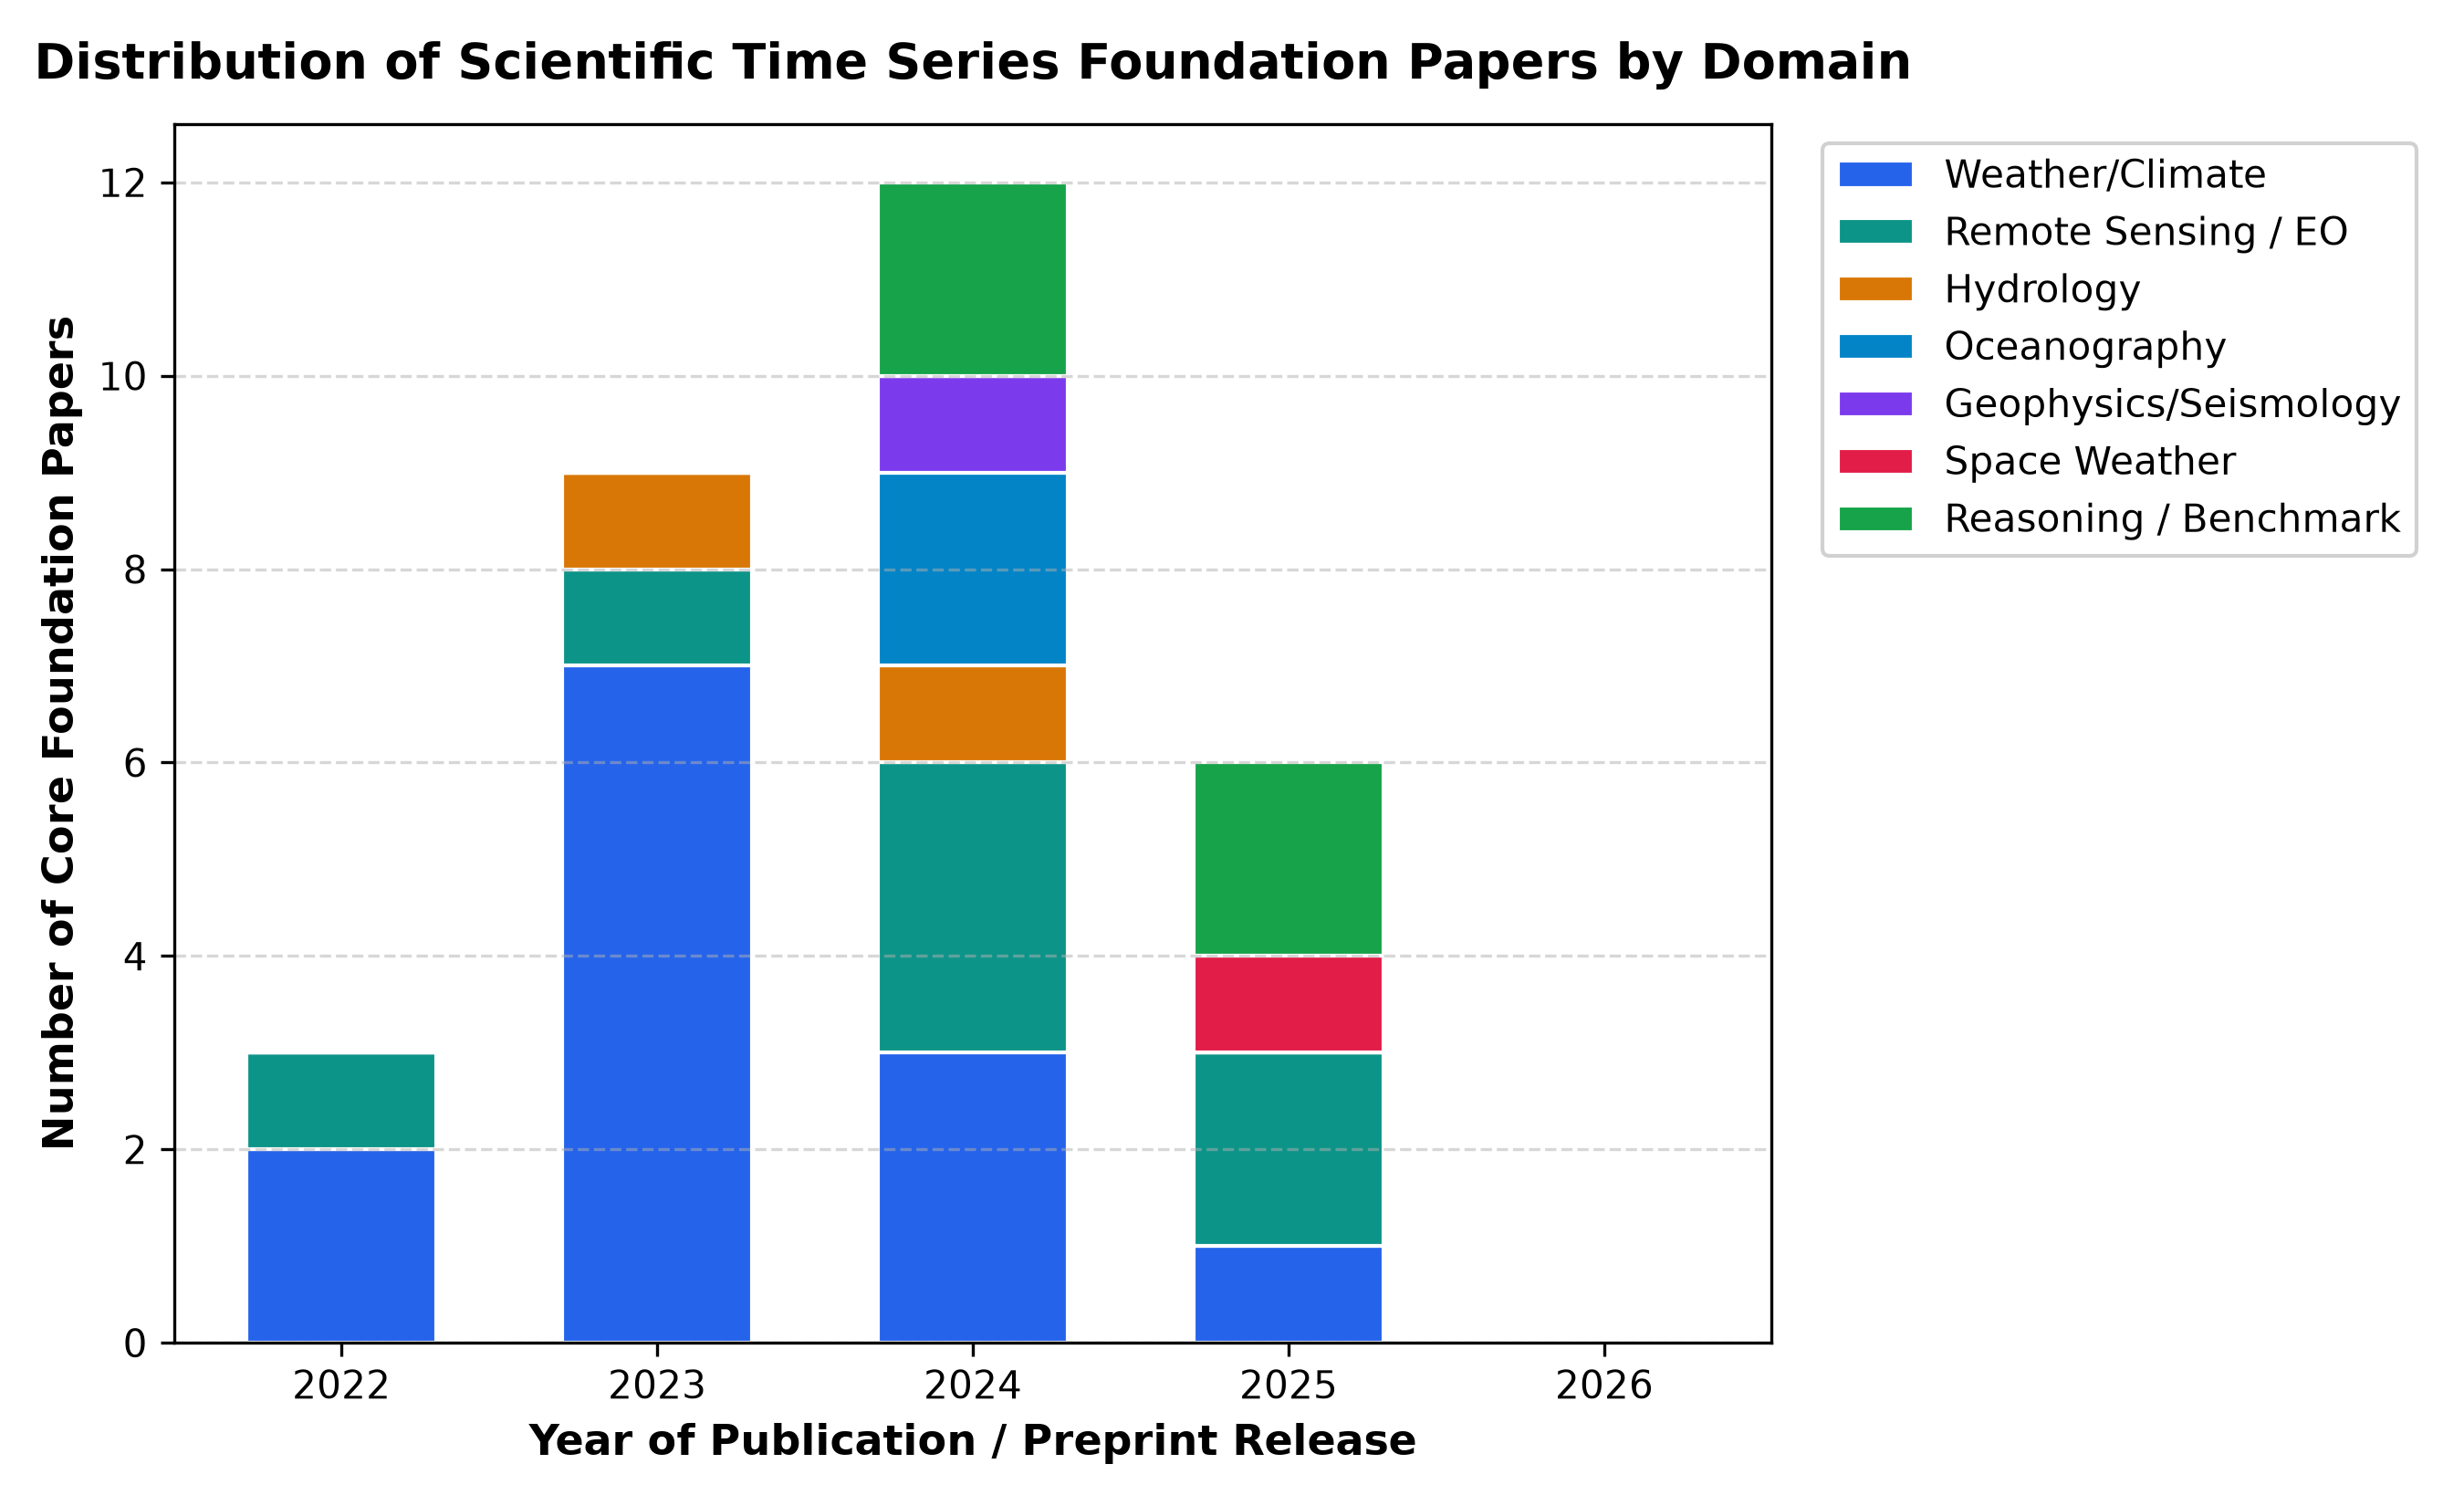
\includegraphics[width=\columnwidth]{figures/publications_by_year.png}
\caption{Annual distribution of scientific time series foundation models and reasoning systems from 2022 to 2026, categorized by scientific domain.}
\label{fig:pubs_by_year}
\end{figure}

As shown in Fig.~\ref{fig:pubs_by_year}, while weather and climate models initiated the initial surge in 2022--2023, the frontier in 2024--2026 has rapidly expanded into cross-disciplinary Earth observation, hydrology, space weather, and autonomous reasoning agents.
